\documentclass[11pt,a4paper]{article}

% Packages
\usepackage[utf8]{inputenc}
\usepackage[T1]{fontenc}
\usepackage[margin=2.5cm]{geometry}
\usepackage{graphicx}
\usepackage{xcolor}
\usepackage{tikz}
\usetikzlibrary{shapes.geometric, arrows.meta, positioning, calc, fit, backgrounds, decorations.pathreplacing, shadows}
\usepackage{pgfplots}
\pgfplotsset{compat=1.18}
\usepackage{listings}
\usepackage{hyperref}
\usepackage{booktabs}
\usepackage{longtable}
\usepackage{enumitem}
\usepackage{fancyhdr}
\usepackage{titlesec}
\usepackage{tocloft}
\usepackage{amsmath}
\usepackage{amssymb}
\usepackage{float}
\usepackage{subcaption}
\usepackage{tcolorbox}

% Colors
\definecolor{primary}{RGB}{41, 128, 185}
\definecolor{secondary}{RGB}{52, 73, 94}
\definecolor{accent}{RGB}{231, 76, 60}
\definecolor{success}{RGB}{39, 174, 96}
\definecolor{warning}{RGB}{241, 196, 15}
\definecolor{codebackground}{RGB}{248, 248, 248}
\definecolor{codeborder}{RGB}{200, 200, 200}

% TikZ styles
\tikzstyle{component} = [rectangle, rounded corners, minimum width=3cm, minimum height=1cm, text centered, draw=primary, fill=primary!10, font=\small]
\tikzstyle{server} = [rectangle, rounded corners, minimum width=2.5cm, minimum height=0.8cm, text centered, draw=success, fill=success!10, font=\small]
\tikzstyle{client} = [rectangle, rounded corners, minimum width=2.5cm, minimum height=0.8cm, text centered, draw=accent, fill=accent!10, font=\small]
\tikzstyle{monitor} = [rectangle, rounded corners, minimum width=2.5cm, minimum height=0.8cm, text centered, draw=warning, fill=warning!10, font=\small]
\tikzstyle{arrow} = [thick,->,>=Stealth]
\tikzstyle{biarrow} = [thick,<->,>=Stealth]
\tikzstyle{dashedarrow} = [thick,->,>=Stealth,dashed]
\tikzstyle{container} = [rectangle, draw=secondary, dashed, inner sep=10pt]

% Code listing style
\lstdefinestyle{yaml}{
    backgroundcolor=\color{codebackground},
    basicstyle=\ttfamily\footnotesize,
    breakatwhitespace=false,
    breaklines=true,
    captionpos=b,
    commentstyle=\color{gray},
    frame=single,
    keepspaces=true,
    keywordstyle=\color{primary}\bfseries,
    numbers=left,
    numbersep=5pt,
    numberstyle=\tiny\color{gray},
    rulecolor=\color{codeborder},
    showspaces=false,
    showstringspaces=false,
    showtabs=false,
    stringstyle=\color{success},
    tabsize=2,
}

\lstdefinestyle{python}{
    backgroundcolor=\color{codebackground},
    basicstyle=\ttfamily\footnotesize,
    breakatwhitespace=false,
    breaklines=true,
    captionpos=b,
    commentstyle=\color{gray}\itshape,
    frame=single,
    keepspaces=true,
    keywordstyle=\color{primary}\bfseries,
    language=Python,
    numbers=left,
    numbersep=5pt,
    numberstyle=\tiny\color{gray},
    rulecolor=\color{codeborder},
    showspaces=false,
    showstringspaces=false,
    showtabs=false,
    stringstyle=\color{success},
    tabsize=4,
}

\lstdefinestyle{bash}{
    backgroundcolor=\color{codebackground},
    basicstyle=\ttfamily\footnotesize,
    breakatwhitespace=false,
    breaklines=true,
    captionpos=b,
    commentstyle=\color{gray},
    frame=single,
    keepspaces=true,
    keywordstyle=\color{primary}\bfseries,
    language=bash,
    numbers=none,
    rulecolor=\color{codeborder},
    showspaces=false,
    showstringspaces=false,
    showtabs=false,
    stringstyle=\color{success},
    tabsize=2,
}

% Placeholder box
\newtcolorbox{placeholder}[1][]{
    colback=yellow!20,
    colframe=orange!75!black,
    fonttitle=\bfseries,
    title={PLACEHOLDER: #1},
    sharp corners,
    boxrule=2pt
}

% Header and footer
\pagestyle{fancy}
\fancyhf{}
\fancyhead[L]{\leftmark}
\fancyhead[R]{HPC Benchmark Toolkit}
\fancyfoot[C]{\thepage}
\renewcommand{\headrulewidth}{0.4pt}
\renewcommand{\footrulewidth}{0.4pt}

% Hyperref setup
\hypersetup{
    colorlinks=true,
    linkcolor=primary,
    filecolor=accent,
    urlcolor=primary,
    citecolor=success,
}

% Title formatting
\titleformat{\section}
{\normalfont\Large\bfseries\color{primary}}{\thesection}{1em}{}
\titleformat{\subsection}
{\normalfont\large\bfseries\color{secondary}}{\thesubsection}{1em}{}
\titleformat{\subsubsection}
{\normalfont\normalsize\bfseries\color{secondary}}{\thesubsubsection}{1em}{}

\begin{document}

% Title Page
\begin{titlepage}
    \centering
    \vspace*{2cm}

    {\Huge\bfseries HPC Benchmark Toolkit\\[0.5cm]}
    {\Large\itshape Technical Report\\[1cm]}

    \vspace{2cm}

    {\Large A Comprehensive Framework for Benchmarking\\LLM Inference Services on HPC Clusters\\[1cm]}

    \vfill

    {\large
    \begin{tabular}{ll}
        \textbf{Target Platform:} & MeluXina HPC Cluster \\
        \textbf{Container Runtime:} & Apptainer/Singularity \\
        \textbf{Scheduler:} & Slurm \\
        \textbf{Services:} & Ollama, vLLM (Single \& Distributed) \\
    \end{tabular}
    }

    \vspace{2cm}

    {\large December 2024}
\end{titlepage}

% Table of Contents
\tableofcontents
\newpage

% ============================================================================
\section{Introduction}
% ============================================================================

\subsection{Project Overview}

The HPC Benchmark Toolkit is a production-ready framework designed for benchmarking Large Language Model (LLM) inference services on High-Performance Computing (HPC) clusters. The toolkit addresses the critical need for reproducible, scalable, and observable benchmarking in enterprise AI deployments.

\subsubsection{Motivation}

Modern AI deployments require careful performance characterization before production rollout. Key challenges include:

\begin{itemize}
    \item \textbf{Reproducibility}: Experiments must be repeatable with identical configurations
    \item \textbf{Scalability}: Benchmarks must scale from single-node to multi-node distributed setups
    \item \textbf{Observability}: Real-time metrics are essential for performance analysis
    \item \textbf{HPC Integration}: Seamless integration with Slurm and containerized workloads
\end{itemize}

\subsubsection{Key Features}

\begin{table}[H]
\centering
\begin{tabular}{@{}lp{10cm}@{}}
\toprule
\textbf{Feature} & \textbf{Description} \\
\midrule
Multi-Service Support & Ollama, vLLM (single and distributed), extensible architecture \\
Distributed Benchmarking & Multi-node server/client orchestration with Ray \\
Real-Time Monitoring & Prometheus/Grafana integration with live dashboards \\
Recipe-Driven & YAML configurations for reproducible experiments \\
HPC-Optimized & Slurm integration, Apptainer container support \\
Comprehensive Metrics & Latency (p50/p90/p99), throughput, resource utilization \\
\bottomrule
\end{tabular}
\caption{Key features of the HPC Benchmark Toolkit}
\end{table}

\subsection{Supported Services}

The toolkit currently supports the following inference services:

\begin{table}[H]
\centering
\begin{tabular}{@{}llll@{}}
\toprule
\textbf{Service} & \textbf{Description} & \textbf{Default Port} & \textbf{API Type} \\
\midrule
Ollama & Local LLM inference server & 11434 & REST \\
vLLM & High-throughput LLM serving & 8000 & OpenAI-compatible \\
vLLM Distributed & Multi-node vLLM with Ray & 8000 & OpenAI-compatible \\
Dummy & Template for custom services & 5000 & REST \\
\bottomrule
\end{tabular}
\caption{Supported inference services}
\end{table}

% ============================================================================
\section{System Architecture}
% ============================================================================

\subsection{High-Level Architecture}

The system follows a modular architecture with clear separation of concerns. Figure~\ref{fig:high-level-arch} illustrates the high-level component structure.

\begin{figure}[H]
\centering
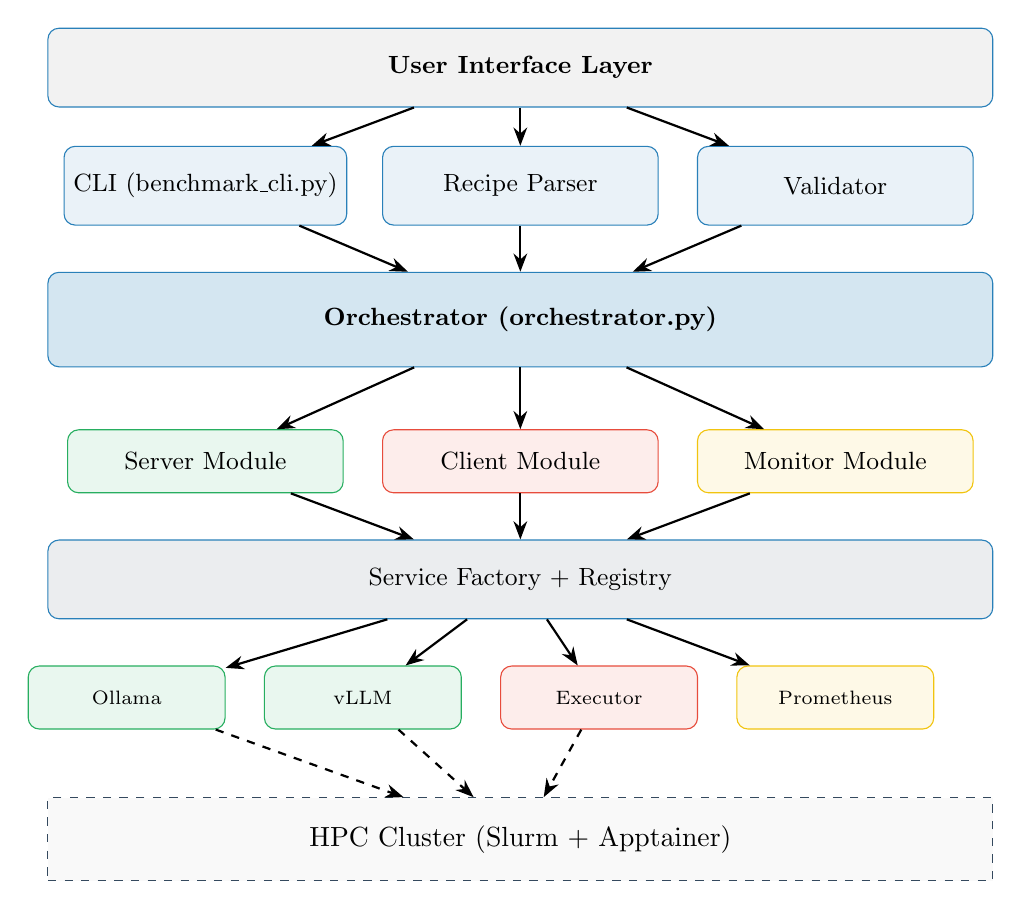
\begin{tikzpicture}[node distance=1.5cm and 2cm]
    % User layer
    \node[component, minimum width=12cm, fill=gray!10] (user) at (0, 5) {\textbf{User Interface Layer}};

    % Interface components
    \node[component, minimum width=3.5cm] (cli) at (-4, 3.5) {CLI (benchmark\_cli.py)};
    \node[component, minimum width=3.5cm] (recipe) at (0, 3.5) {Recipe Parser};
    \node[component, minimum width=3.5cm] (validator) at (4, 3.5) {Validator};

    % Orchestrator
    \node[component, minimum width=12cm, minimum height=1.2cm, fill=primary!20] (orch) at (0, 1.8) {\textbf{Orchestrator (orchestrator.py)}};

    % Core modules
    \node[server, minimum width=3.5cm] (servers) at (-4, 0) {Server Module};
    \node[client, minimum width=3.5cm] (clients) at (0, 0) {Client Module};
    \node[monitor, minimum width=3.5cm] (monitors) at (4, 0) {Monitor Module};

    % Service Factory
    \node[component, minimum width=12cm, fill=secondary!10] (factory) at (0, -1.5) {Service Factory + Registry};

    % Implementations
    \node[server, minimum width=2.5cm, font=\scriptsize] (ollama) at (-5, -3) {Ollama};
    \node[server, minimum width=2.5cm, font=\scriptsize] (vllm) at (-2, -3) {vLLM};
    \node[client, minimum width=2.5cm, font=\scriptsize] (exec1) at (1, -3) {Executor};
    \node[monitor, minimum width=2.5cm, font=\scriptsize] (prom) at (4, -3) {Prometheus};

    % Cluster layer
    \node[container, minimum width=12cm, minimum height=1cm, fill=gray!5] (cluster) at (0, -4.8) {HPC Cluster (Slurm + Apptainer)};

    % Arrows
    \draw[arrow] (user) -- (cli);
    \draw[arrow] (user) -- (recipe);
    \draw[arrow] (user) -- (validator);
    \draw[arrow] (cli) -- (orch);
    \draw[arrow] (recipe) -- (orch);
    \draw[arrow] (validator) -- (orch);
    \draw[arrow] (orch) -- (servers);
    \draw[arrow] (orch) -- (clients);
    \draw[arrow] (orch) -- (monitors);
    \draw[arrow] (servers) -- (factory);
    \draw[arrow] (clients) -- (factory);
    \draw[arrow] (monitors) -- (factory);
    \draw[arrow] (factory) -- (ollama);
    \draw[arrow] (factory) -- (vllm);
    \draw[arrow] (factory) -- (exec1);
    \draw[arrow] (factory) -- (prom);
    \draw[dashedarrow] (ollama) -- (cluster);
    \draw[dashedarrow] (vllm) -- (cluster);
    \draw[dashedarrow] (exec1) -- (cluster);
\end{tikzpicture}
\caption{High-level system architecture}
\label{fig:high-level-arch}
\end{figure}

\subsection{Design Patterns}

The toolkit employs several software design patterns to ensure maintainability and extensibility:

\subsubsection{Factory Pattern}

The \texttt{ServiceFactory} class provides dynamic component instantiation based on service type:

\begin{lstlisting}[style=python, caption={ServiceFactory implementation pattern}]
class ServiceFactory:
    _registry = {}

    @classmethod
    def register_service(cls, name, server_cls, controller_cls, executor_cls):
        cls._registry[name] = {
            'server': server_cls,
            'controller': controller_cls,
            'executor': executor_cls
        }

    @classmethod
    def create_server_manager(cls, service_name, config):
        return cls._registry[service_name]['server'](config)
\end{lstlisting}

\subsubsection{Template Method Pattern}

Base classes define algorithm skeletons while subclasses provide specific implementations:

\begin{figure}[H]
\centering
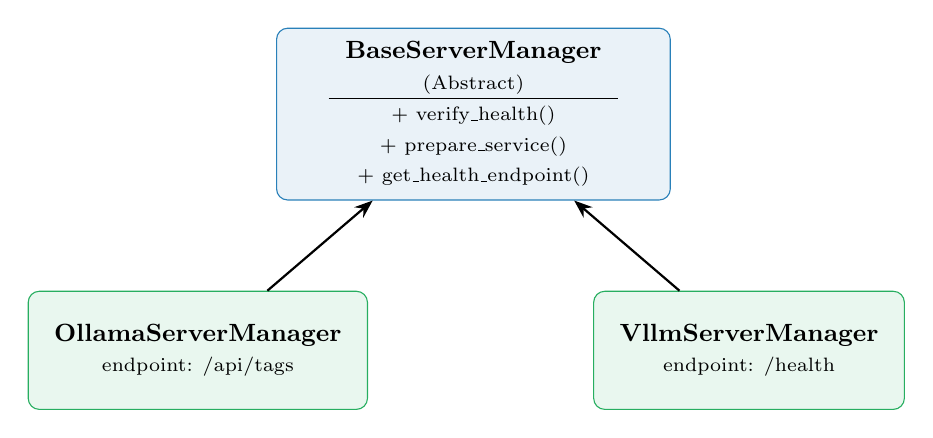
\begin{tikzpicture}[node distance=2cm]
    % Base class
    \node[component, minimum width=5cm, minimum height=2cm] (base) at (0, 2) {
        \begin{tabular}{c}
            \textbf{BaseServerManager} \\
            \scriptsize (Abstract) \\
            \hline
            \scriptsize + verify\_health() \\
            \scriptsize + prepare\_service() \\
            \scriptsize + get\_health\_endpoint()
        \end{tabular}
    };

    % Concrete classes
    \node[server, minimum width=3.5cm, minimum height=1.5cm] (ollama) at (-3.5, -1) {
        \begin{tabular}{c}
            \textbf{OllamaServerManager} \\
            \scriptsize endpoint: /api/tags
        \end{tabular}
    };

    \node[server, minimum width=3.5cm, minimum height=1.5cm] (vllm) at (3.5, -1) {
        \begin{tabular}{c}
            \textbf{VllmServerManager} \\
            \scriptsize endpoint: /health
        \end{tabular}
    };

    % Inheritance arrows
    \draw[arrow] (ollama) -- (base);
    \draw[arrow] (vllm) -- (base);
\end{tikzpicture}
\caption{Template Method Pattern in Server Managers}
\end{figure}

\subsection{Component Details}

\subsubsection{Server Managers}

Server managers handle the lifecycle of inference services:

\begin{itemize}
    \item \textbf{Health Checking}: Polls service endpoints to verify readiness
    \item \textbf{Service Preparation}: Loads models, initializes resources
    \item \textbf{Configuration Parsing}: Extracts service-specific settings from recipes
\end{itemize}

\begin{table}[H]
\centering
\begin{tabular}{@{}llll@{}}
\toprule
\textbf{Manager} & \textbf{Health Endpoint} & \textbf{Port} & \textbf{Special Features} \\
\midrule
OllamaServerManager & /api/tags & 11434 & Model pulling via /api/pull \\
VllmServerManager & /health & 8000 & Ray cluster integration \\
DummyServerManager & /health & 5000 & Template implementation \\
\bottomrule
\end{tabular}
\caption{Server Manager implementations}
\end{table}

\subsubsection{Workload Controllers}

Controllers coordinate workload execution across client nodes:

\begin{figure}[H]
\centering
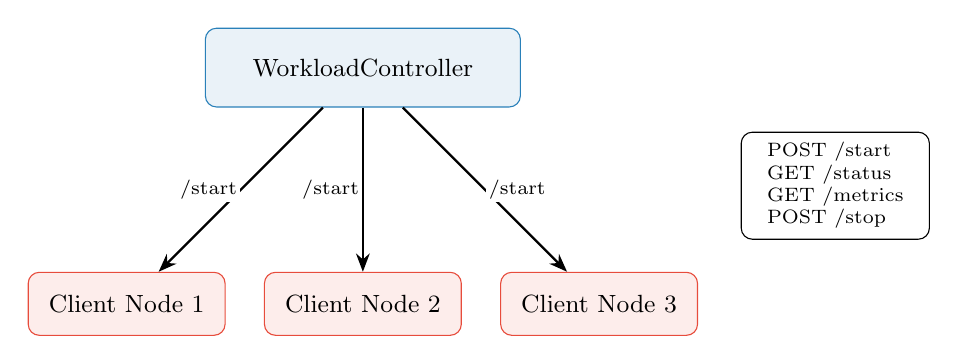
\begin{tikzpicture}[node distance=1.5cm]
    % Controller
    \node[component, minimum width=4cm] (ctrl) at (0, 3) {WorkloadController};

    % Client nodes
    \node[client, minimum width=2.5cm] (c1) at (-3, 0) {Client Node 1};
    \node[client, minimum width=2.5cm] (c2) at (0, 0) {Client Node 2};
    \node[client, minimum width=2.5cm] (c3) at (3, 0) {Client Node 3};

    % Arrows with methods
    \draw[arrow] (ctrl) -- node[left, font=\scriptsize, fill=white, inner sep=1pt] {/start} (c1);
    \draw[arrow] (ctrl) -- node[left, font=\scriptsize, fill=white, inner sep=1pt] {/start} (c2);
    \draw[arrow] (ctrl) -- node[right, font=\scriptsize, fill=white, inner sep=1pt] {/start} (c3);

    % Method list
    \node[draw, rounded corners, fill=white, font=\scriptsize] at (6, 1.5) {
        \begin{tabular}{l}
            POST /start \\
            GET /status \\
            GET /metrics \\
            POST /stop
        \end{tabular}
    };
\end{tikzpicture}
\caption{Workload Controller to Client communication}
\end{figure}

\subsubsection{Workload Executors}

Executors run on client nodes as Flask servers, executing the actual benchmark workload:

\begin{lstlisting}[style=python, caption={Workload Executor REST API}]
# Flask endpoints exposed by each executor
GET  /health              # Check executor status
POST /start               # Start workload with JSON config
GET  /status              # Get current workload status
GET  /metrics             # Fetch collected metrics
GET  /metrics/prometheus  # Prometheus-compatible format
POST /stop                # Stop workload execution
\end{lstlisting}

% ============================================================================
\section{Communication Architecture}
% ============================================================================

\subsection{Overview}

The toolkit employs a hybrid communication architecture combining:
\begin{itemize}
    \item \textbf{REST/HTTP}: Control plane communication between orchestrator and components
    \item \textbf{Service APIs}: Data plane communication between clients and inference servers
    \item \textbf{Prometheus Push/Pull}: Metrics collection and aggregation
\end{itemize}

\subsection{Control Plane Communication}

\begin{figure}[H]
\centering
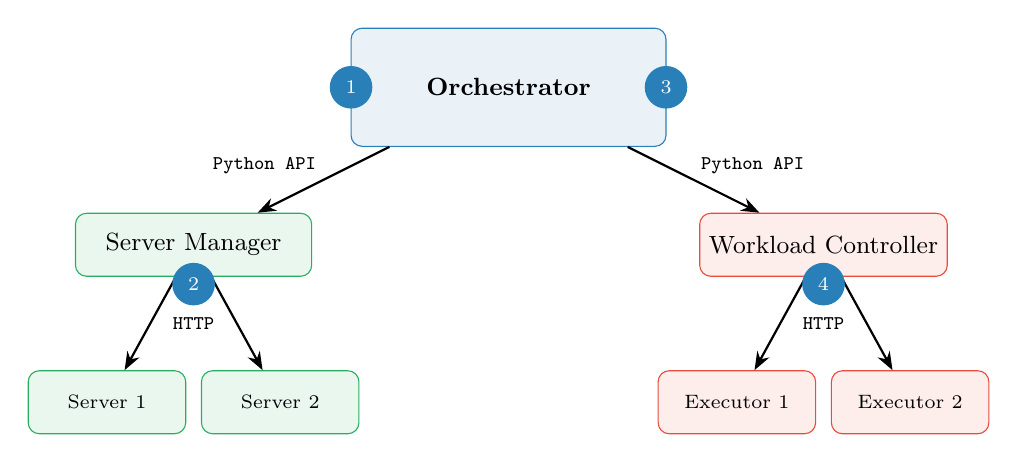
\begin{tikzpicture}[node distance=2cm]
    % Orchestrator
    \node[component, minimum width=4cm, minimum height=1.5cm] (orch) at (0, 4) {\textbf{Orchestrator}};

    % Server Manager
    \node[server, minimum width=3cm] (sm) at (-4, 2) {Server Manager};

    % Workload Controller
    \node[client, minimum width=3cm] (wc) at (4, 2) {Workload Controller};

    % Server nodes
    \node[server, minimum width=2cm, font=\scriptsize] (s1) at (-5.1, 0) {Server 1};
    \node[server, minimum width=2cm, font=\scriptsize] (s2) at (-2.9, 0) {Server 2};

    % Client executors
    \node[client, minimum width=2cm, font=\scriptsize] (e1) at (2.9, 0) {Executor 1};
    \node[client, minimum width=2cm, font=\scriptsize] (e2) at (5.1, 0) {Executor 2};

    % Protocol labels
    \node[fill=white, font=\scriptsize\ttfamily] at (-3.1, 3) {Python API};
    \node[fill=white, font=\scriptsize\ttfamily] at (3.1, 3) {Python API};
    \node[fill=white, font=\scriptsize\ttfamily] at (-4, 1) {HTTP};
    \node[fill=white, font=\scriptsize\ttfamily] at (4, 1) {HTTP};

    % Arrows
    \draw[arrow] (orch) -- (sm);
    \draw[arrow] (orch) -- (wc);
    \draw[arrow] (sm) -- (s1);
    \draw[arrow] (sm) -- (s2);
    \draw[arrow] (wc) -- (e1);
    \draw[arrow] (wc) -- (e2);

    % Sequence numbers
    \node[circle, fill=primary, text=white, font=\scriptsize] at (-2, 4) {1};
    \node[circle, fill=primary, text=white, font=\scriptsize] at (-4, 1.5) {2};
    \node[circle, fill=primary, text=white, font=\scriptsize] at (2, 4) {3};
    \node[circle, fill=primary, text=white, font=\scriptsize] at (4, 1.5) {4};
\end{tikzpicture}
\caption{Control plane communication flow}
\label{fig:control-plane}
\end{figure}

\subsection{Data Plane Communication}

During benchmark execution, clients send inference requests directly to servers:

\begin{figure}[H]
\centering
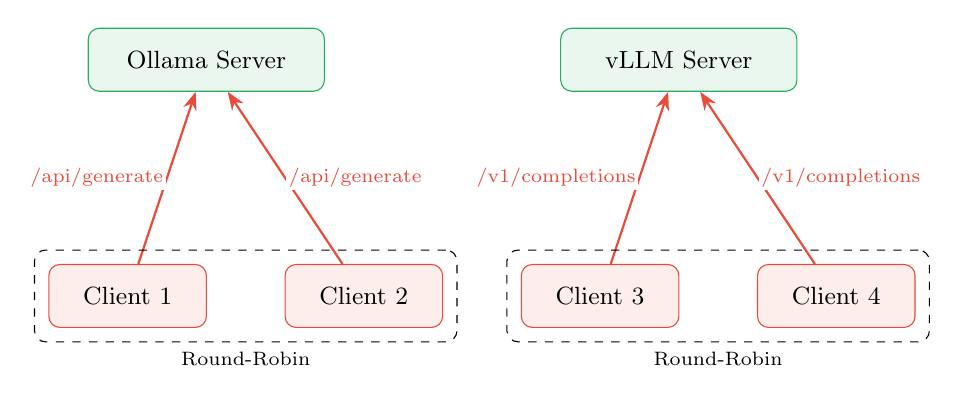
\begin{tikzpicture}[node distance=2cm]
    % Servers
    \node[server, minimum width=3cm] (s1) at (-3, 2) {Ollama Server};
    \node[server, minimum width=3cm] (s2) at (3, 2) {vLLM Server};

    % Clients
    \node[client, minimum width=2cm] (c1) at (-4, -1) {Client 1};
    \node[client, minimum width=2cm] (c2) at (-1, -1) {Client 2};
    \node[client, minimum width=2cm] (c3) at (2, -1) {Client 3};
    \node[client, minimum width=2cm] (c4) at (5, -1) {Client 4};

    % Request arrows
    \draw[arrow, accent] (c1) -- node[left, font=\scriptsize, fill=white, inner sep=1pt] {/api/generate} (s1);
    \draw[arrow, accent] (c2) -- node[right, font=\scriptsize, fill=white, inner sep=1pt] {/api/generate} (s1);
    \draw[arrow, accent] (c3) -- node[left, font=\scriptsize, fill=white, inner sep=1pt] {/v1/completions} (s2);
    \draw[arrow, accent] (c4) -- node[right, font=\scriptsize, fill=white, inner sep=1pt] {/v1/completions} (s2);

    % Load distribution label
    \node[draw, dashed, rounded corners, fit=(c1)(c2), inner sep=5pt, label=below:{\scriptsize Round-Robin}] {};
    \node[draw, dashed, rounded corners, fit=(c3)(c4), inner sep=5pt, label=below:{\scriptsize Round-Robin}] {};
\end{tikzpicture}
\caption{Data plane: Client to Server inference requests}
\end{figure}

\subsection{Metrics Collection Pipeline}

\begin{figure}[H]
\centering
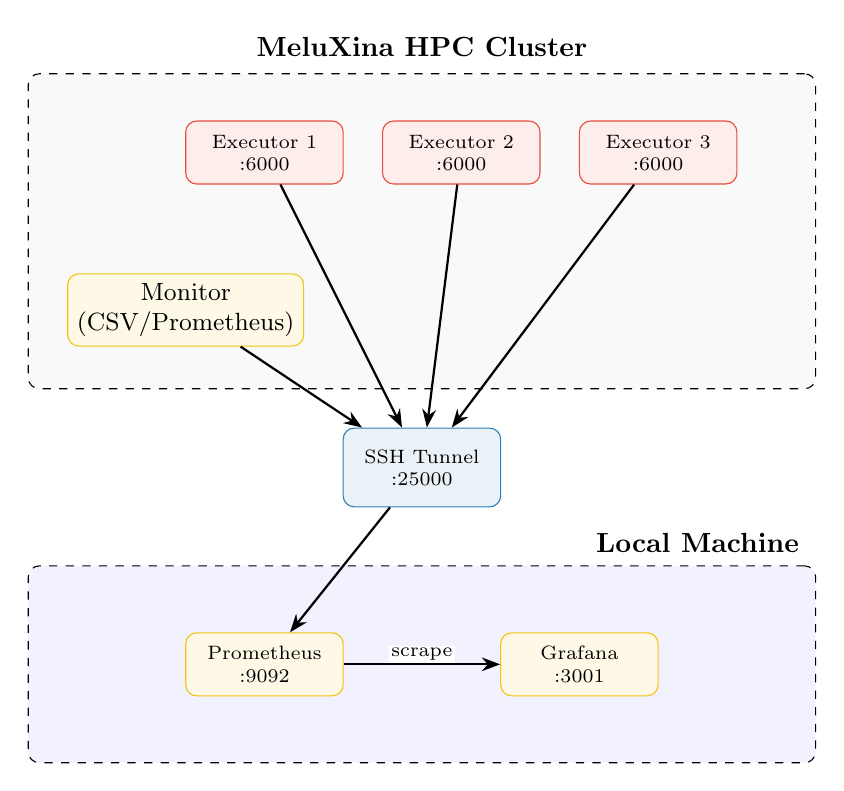
\begin{tikzpicture}[node distance=1.5cm]
    % HPC Cluster boundary
    \begin{scope}[on background layer]
        \node[draw, dashed, rounded corners, minimum width=10cm, minimum height=4cm, fill=gray!5] (hpc) at (0, 2) {};
        \node[above] at (0, 4.1) {\textbf{MeluXina HPC Cluster}};
    \end{scope}

    % Executors
    \node[client, minimum width=2cm, font=\scriptsize, align=center] (e1) at (-2, 3) {Executor 1\\:6000};
    \node[client, minimum width=2cm, font=\scriptsize, align=center] (e2) at (0.5, 3) {Executor 2\\:6000};
    \node[client, minimum width=2cm, font=\scriptsize, align=center] (e3) at (3, 3) {Executor 3\\:6000};

    % Monitor
    \node[monitor, minimum width=2.5cm, align=center] (mon) at (-3, 1) {Monitor\\(CSV/Prometheus)};

    % SSH Tunnel
    \node[component, minimum width=2cm, font=\scriptsize, align=center] (tunnel) at (0, -1) {SSH Tunnel\\:25000};

    % Laptop boundary
    \begin{scope}[on background layer]
        \node[draw, dashed, rounded corners, minimum width=10cm, minimum height=2.5cm, fill=blue!5] (laptop) at (0, -3.5) {};
        \node[above] at (3.5, -2.2) {\textbf{Local Machine}};
    \end{scope}

    % Prometheus & Grafana
    \node[monitor, minimum width=2cm, font=\scriptsize, align=center] (prom) at (-2, -3.5) {Prometheus\\:9092};
    \node[monitor, minimum width=2cm, font=\scriptsize, align=center] (grafana) at (2, -3.5) {Grafana\\:3001};

    % Arrows
    \draw[arrow] (e1) -- (tunnel);
    \draw[arrow] (e2) -- (tunnel);
    \draw[arrow] (e3) -- (tunnel);
    \draw[arrow] (mon) -- (tunnel);
    \draw[arrow] (tunnel) -- (prom);
    \draw[arrow] (prom) -- node[above, font=\scriptsize, fill=white, inner sep=1pt] {scrape} (grafana);

\end{tikzpicture}
\caption{Metrics collection pipeline with SSH tunneling}
\label{fig:metrics-pipeline}
\end{figure}

\subsection{Message Sequence Diagram}

\begin{figure}[H]
\centering
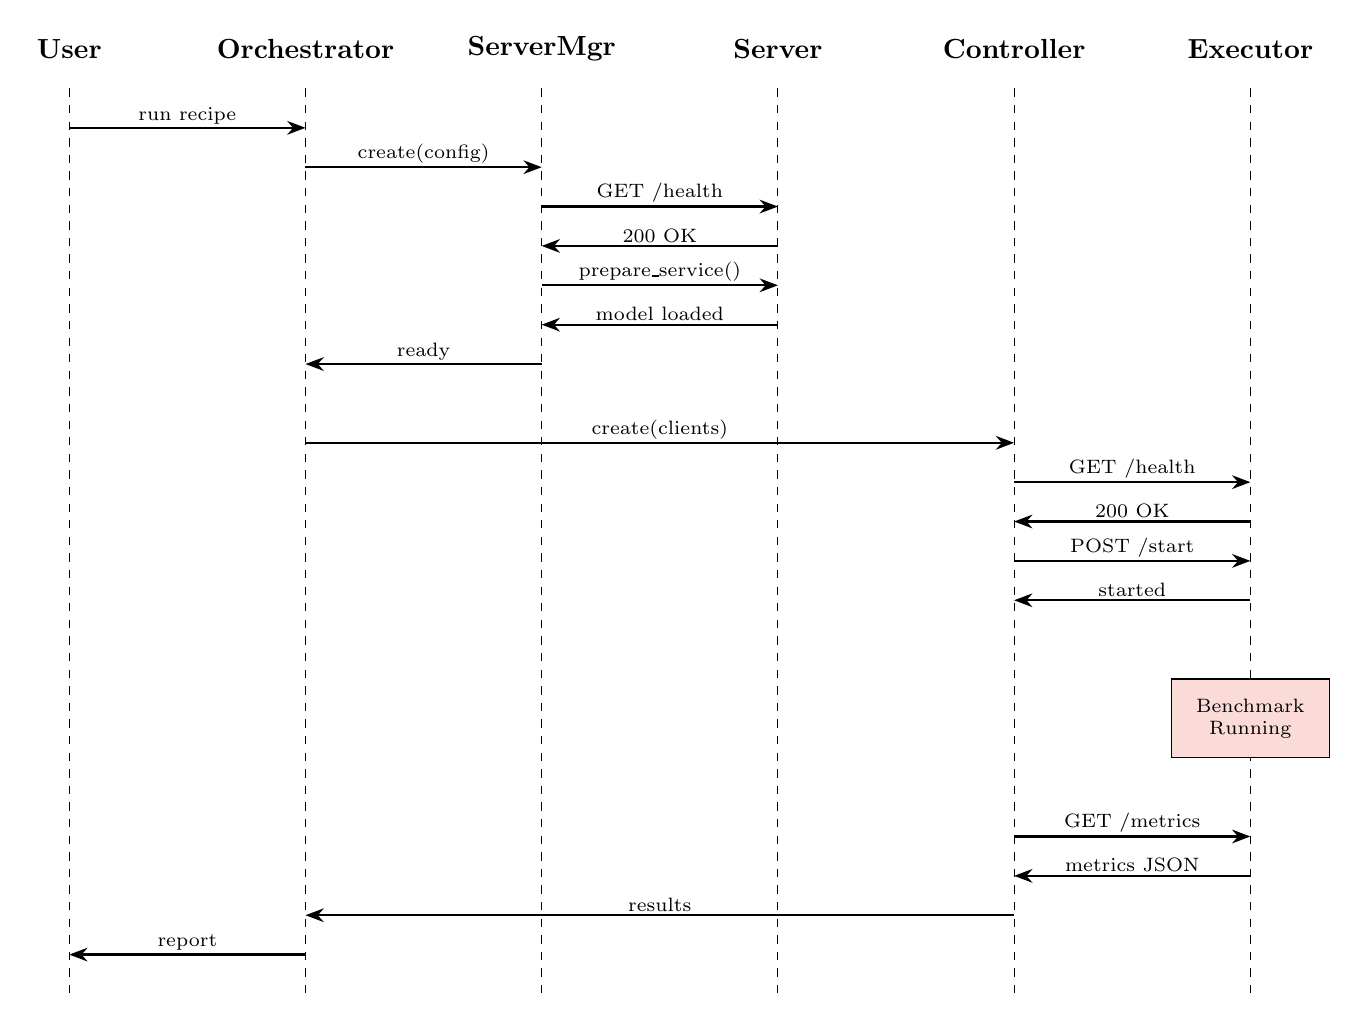
\begin{tikzpicture}[node distance=0.5cm]
    % Participants
    \node (user) at (0, 0) {\textbf{User}};
    \node (orch) at (3, 0) {\textbf{Orchestrator}};
    \node (sm) at (6, 0) {\textbf{ServerMgr}};
    \node (server) at (9, 0) {\textbf{Server}};
    \node (wc) at (12, 0) {\textbf{Controller}};
    \node (exec) at (15, 0) {\textbf{Executor}};

    % Lifelines
    \draw[dashed] (0, -0.5) -- (0, -12);
    \draw[dashed] (3, -0.5) -- (3, -12);
    \draw[dashed] (6, -0.5) -- (6, -12);
    \draw[dashed] (9, -0.5) -- (9, -12);
    \draw[dashed] (12, -0.5) -- (12, -12);
    \draw[dashed] (15, -0.5) -- (15, -12);

    % Messages
    \draw[arrow] (0, -1) -- node[above, font=\scriptsize, fill=white, inner sep=1pt] {run recipe} (3, -1);
    \draw[arrow] (3, -1.5) -- node[above, font=\scriptsize, fill=white, inner sep=1pt] {create(config)} (6, -1.5);
    \draw[arrow] (6, -2) -- node[above, font=\scriptsize, fill=white, inner sep=1pt] {GET /health} (9, -2);
    \draw[arrow] (9, -2.5) -- node[above, font=\scriptsize, fill=white, inner sep=1pt] {200 OK} (6, -2.5);
    \draw[arrow] (6, -3) -- node[above, font=\scriptsize, fill=white, inner sep=1pt] {prepare\_service()} (9, -3);
    \draw[arrow] (9, -3.5) -- node[above, font=\scriptsize, fill=white, inner sep=1pt] {model loaded} (6, -3.5);
    \draw[arrow] (6, -4) -- node[above, font=\scriptsize, fill=white, inner sep=1pt] {ready} (3, -4);

    \draw[arrow] (3, -5) -- node[above, font=\scriptsize, fill=white, inner sep=1pt] {create(clients)} (12, -5);
    \draw[arrow] (12, -5.5) -- node[above, font=\scriptsize, fill=white, inner sep=1pt] {GET /health} (15, -5.5);
    \draw[arrow] (15, -6) -- node[above, font=\scriptsize, fill=white, inner sep=1pt] {200 OK} (12, -6);
    \draw[arrow] (12, -6.5) -- node[above, font=\scriptsize, fill=white, inner sep=1pt] {POST /start} (15, -6.5);
    \draw[arrow] (15, -7) -- node[above, font=\scriptsize, fill=white, inner sep=1pt] {started} (12, -7);

    % Benchmark execution
    \node[draw, fill=accent!20, minimum width=2cm, minimum height=1cm, font=\scriptsize, align=center] at (15, -8.5) {Benchmark\\Running};

    \draw[arrow] (12, -10) -- node[above, font=\scriptsize, fill=white, inner sep=1pt] {GET /metrics} (15, -10);
    \draw[arrow] (15, -10.5) -- node[above, font=\scriptsize, fill=white, inner sep=1pt] {metrics JSON} (12, -10.5);
    \draw[arrow] (12, -11) -- node[above, font=\scriptsize, fill=white, inner sep=1pt] {results} (3, -11);
    \draw[arrow] (3, -11.5) -- node[above, font=\scriptsize, fill=white, inner sep=1pt] {report} (0, -11.5);
\end{tikzpicture}
\caption{Message sequence for benchmark execution}
\end{figure}

% ============================================================================
\section{Execution Flow}
% ============================================================================

\subsection{Seven-Phase Execution Model}

The benchmark execution follows a structured seven-phase model:

\begin{figure}[H]
\centering
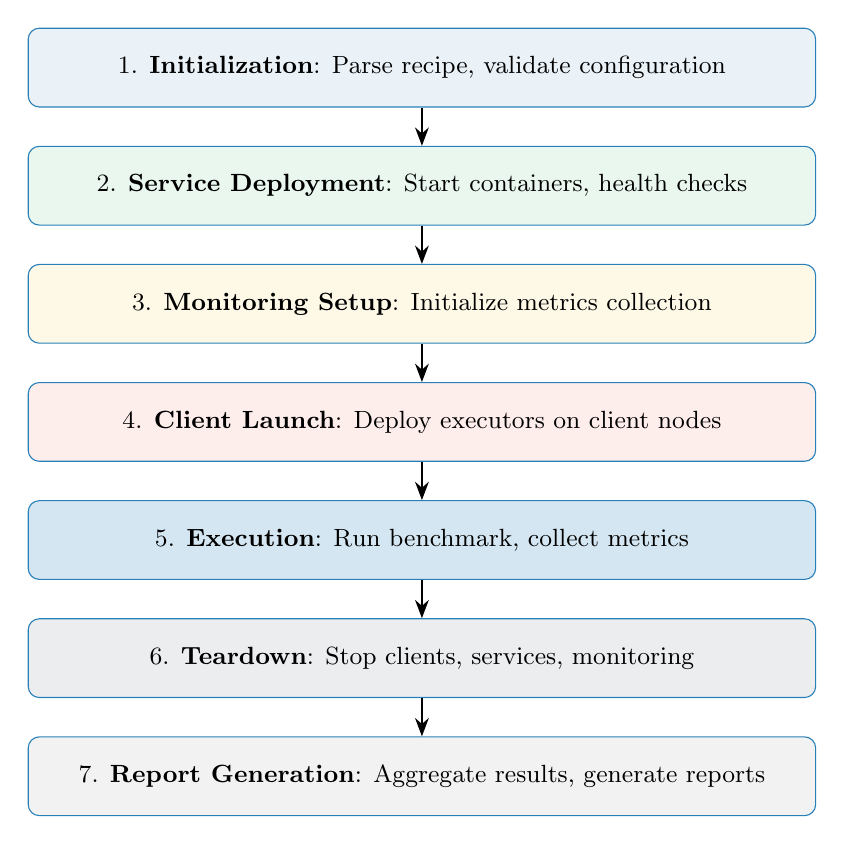
\begin{tikzpicture}[node distance=0.8cm]
    % Phases
    \node[component, minimum width=10cm, fill=primary!10] (p1) at (0, 6) {1. \textbf{Initialization}: Parse recipe, validate configuration};
    \node[component, minimum width=10cm, fill=success!10] (p2) at (0, 4.5) {2. \textbf{Service Deployment}: Start containers, health checks};
    \node[component, minimum width=10cm, fill=warning!10] (p3) at (0, 3) {3. \textbf{Monitoring Setup}: Initialize metrics collection};
    \node[component, minimum width=10cm, fill=accent!10] (p4) at (0, 1.5) {4. \textbf{Client Launch}: Deploy executors on client nodes};
    \node[component, minimum width=10cm, fill=primary!20] (p5) at (0, 0) {5. \textbf{Execution}: Run benchmark, collect metrics};
    \node[component, minimum width=10cm, fill=secondary!10] (p6) at (0, -1.5) {6. \textbf{Teardown}: Stop clients, services, monitoring};
    \node[component, minimum width=10cm, fill=gray!10] (p7) at (0, -3) {7. \textbf{Report Generation}: Aggregate results, generate reports};

    % Arrows
    \draw[arrow] (p1) -- (p2);
    \draw[arrow] (p2) -- (p3);
    \draw[arrow] (p3) -- (p4);
    \draw[arrow] (p4) -- (p5);
    \draw[arrow] (p5) -- (p6);
    \draw[arrow] (p6) -- (p7);
\end{tikzpicture}
\caption{Seven-phase execution model}
\end{figure}

\subsection{Detailed Phase Descriptions}

\subsubsection{Phase 1: Initialization}

\begin{enumerate}
    \item Load and parse YAML recipe file
    \item Validate against JSON schema (\texttt{schemas/recipe-format.yaml})
    \item Expand parameter sweeps (Cartesian product)
    \item Initialize logging and output directories
\end{enumerate}

\subsubsection{Phase 2: Service Deployment}

\begin{enumerate}
    \item Create ServerManager via ServiceFactory
    \item Build endpoint list from server node hostnames
    \item Poll health check endpoints with configurable timeout
    \item Execute service preparation (model loading)
\end{enumerate}

\subsubsection{Phase 3: Monitoring Setup}

This phase sets up the system to track what's happening during the benchmark. It prepares both the HPC cluster and personal laptop to collect performance data:

\begin{enumerate}
    \item \textbf{Start Monitoring}: Turn on the monitor tool that will watch CPU, GPU, and memory usage
    \item \textbf{Choose What to Track}: Decide which metrics to collect (CPU usage, GPU usage, memory, etc.)
    \item \textbf{Connect to Pushgateway}: Set up connection to Prometheus Pushgateway (stores the data)
    \item \textbf{Create Folders}: Make directories to save the collected data as CSV files
    \item \textbf{Run Monitor in Background}: Start monitoring that runs continuously and takes a measurement every 1 second by default
    \item \textbf{Check Grafana Dashboard}: Make sure the dashboard on your laptop is ready to see the data
\end{enumerate}

\textbf{Main Settings:}
\begin{itemize}
    \item \texttt{monitor\_interval}: How often to check the system (example: every 1 second)
    \item \texttt{prometheus\_push\_interval}: How often to send data to storage (example: every 15 seconds)
    \item \texttt{pushgateway\_url}: Where to send the data (example: \texttt{http://mel2109:9091})
    \item \texttt{output\_file}: File name to save results (example: \texttt{benchmark\_metrics.csv})
\end{itemize}

\textbf{Parts of the Monitoring System:}
\begin{itemize}
    \item \textbf{Prometheus on Your Laptop} (port 9092): Collects data every 15 seconds from the HPC cluster
    \item \textbf{Grafana on Your Laptop} (port 3001): Shows graphs and charts of the performance data
    \item \textbf{Pushgateway on HPC}: A storage box that receives metrics from the cluster
    \item \textbf{SSH Tunnels}: Secret paths that let your laptop see the HPC metrics safely
\end{itemize}

\subsubsection{Phase 4: Client Launch}

\begin{enumerate}
    \item Create WorkloadController via ServiceFactory
    \item Verify executor health on all client nodes
    \item Distribute workload configuration
    \item Initialize thread pools on each executor
\end{enumerate}

\subsubsection{Phase 5: Execution}

\begin{enumerate}
    \item Warmup period (configurable duration)
    \item Main benchmark execution
    \item Continuous metrics collection
    \item Real-time Prometheus scraping
\end{enumerate}

\subsubsection{Phase 6: Teardown}

\begin{enumerate}
    \item Send stop signals to all executors
    \item Collect final metrics
    \item Stop monitoring processes
    \item Clean up resources
\end{enumerate}

\subsubsection{Phase 7: Report Generation}

\begin{enumerate}
    \item Aggregate metrics from all clients
    \item Calculate statistics (mean, p50, p90, p99)
    \item Generate CSV/JSON output files
    \item Create summary report
\end{enumerate}

% ============================================================================
\section{Recipe Configuration System}
% ============================================================================

\subsection{Recipe Structure}

Recipes are YAML files that declaratively define benchmark configurations:

\begin{lstlisting}[style=yaml, caption={Complete recipe structure}]
scenario: "experiment-name"
partition: "gpu"
account: "p200981"
qos: "default"

orchestration:
  mode: "slurm"
  total_nodes: 5
  node_allocation:
    servers:
      nodes: 2
    clients:
      nodes: 2
      clients_per_node: 10
    monitors:
      nodes: 1
  job_config:
    time_limit: "02:00:00"
    exclusive: true

resources:
  servers:
    gpus: 2
    cpus_per_task: 1
    mem_gb: 32
  clients:
    gpus: 0
    cpus_per_task: 2
    mem_gb: 16

workload:
  component: "inference"
  service: "ollama"
  duration: "2m"
  warmup: "1m"
  model: "llama2"
  clients_per_node: 10

servers:
  health_check:
    enabled: true
    timeout: 300
    interval: 5
    endpoint: "/api/tags"
  service_config:
    gpu_layers: 0

artifacts:
  containers_dir: "/path/to/containers/"
  service:
    path: "ollama_latest.sif"
  python:
    path: "python_3_12_3_v2.sif"

binds:
  - "/project/.ollama:/root/.ollama:rw"
  - "/project/scratch:/scratch:rw"
\end{lstlisting}

\subsection{Recipe Validation}

\begin{placeholder}{Laura's Section}
Please describe the recipe validation system in detail:
\begin{itemize}
    \item JSON Schema validation implementation
    \item Validation rules and error messages
    \item Custom validators
    \item Schema versioning
    \item Interactive validation mode
\end{itemize}
\end{placeholder}

\subsection{Parameter Sweeps}

The recipe system supports automatic parameter expansion:

\begin{lstlisting}[style=yaml, caption={Parameter sweep configuration}]
workload:
  batch: [1, 4, 8]           # 3 values
  concurrency: [1, 8, 32]    # 3 values
  prompt_len: [128, 512]     # 2 values
  # Total trials: 3 x 3 x 2 = 18
\end{lstlisting}

% ============================================================================
\section{Distributed Benchmarking with Ray}
% ============================================================================

\subsection{Ray Cluster Architecture}

For distributed vLLM deployments, the toolkit integrates with Ray for tensor and pipeline parallelism:

\begin{figure}[H]
\centering
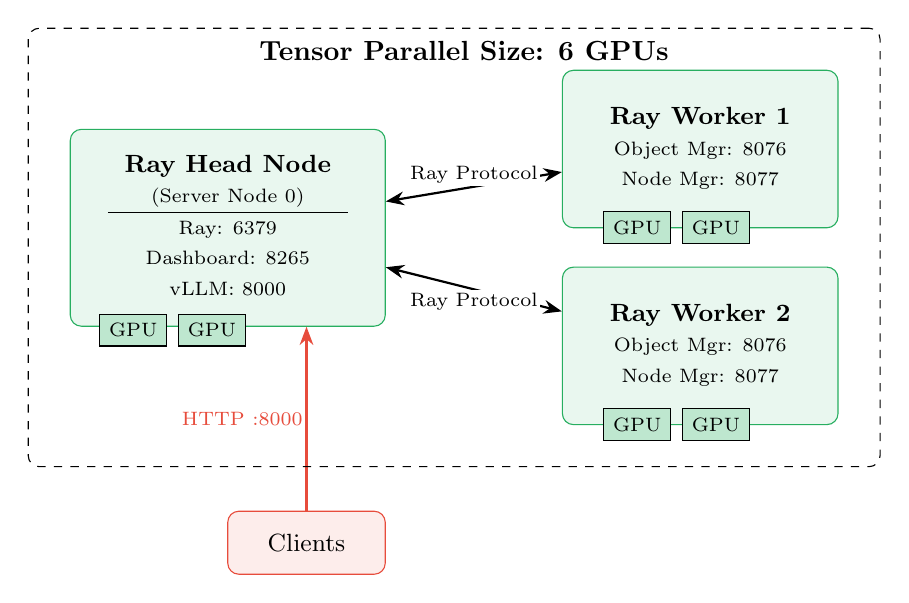
\begin{tikzpicture}[node distance=1.5cm]
    % Ray Head Node
    \node[server, minimum width=4cm, minimum height=2.5cm] (head) at (-3, 0) {
        \begin{tabular}{c}
            \textbf{Ray Head Node} \\
            \scriptsize (Server Node 0) \\
            \hline
            \scriptsize Ray: 6379 \\
            \scriptsize Dashboard: 8265 \\
            \scriptsize vLLM: 8000
        \end{tabular}
    };

    % Ray Worker Nodes
    \node[server, minimum width=3.5cm, minimum height=2cm] (w1) at (3, 1) {
        \begin{tabular}{c}
            \textbf{Ray Worker 1} \\
            \scriptsize Object Mgr: 8076 \\
            \scriptsize Node Mgr: 8077
        \end{tabular}
    };

    \node[server, minimum width=3.5cm, minimum height=2cm] (w2) at (3, -1.5) {
        \begin{tabular}{c}
            \textbf{Ray Worker 2} \\
            \scriptsize Object Mgr: 8076 \\
            \scriptsize Node Mgr: 8077
        \end{tabular}
    };

    % GPU icons
    \node[draw, fill=success!30, minimum width=0.8cm, font=\scriptsize] at (-4.2, -1.3) {GPU};
    \node[draw, fill=success!30, minimum width=0.8cm, font=\scriptsize] at (-3.2, -1.3) {GPU};
    \node[draw, fill=success!30, minimum width=0.8cm, font=\scriptsize] at (2.2, 0) {GPU};
    \node[draw, fill=success!30, minimum width=0.8cm, font=\scriptsize] at (3.2, 0) {GPU};
    \node[draw, fill=success!30, minimum width=0.8cm, font=\scriptsize] at (2.2, -2.5) {GPU};
    \node[draw, fill=success!30, minimum width=0.8cm, font=\scriptsize] at (3.2, -2.5) {GPU};

    % Connections
    \draw[biarrow, thick] (head) -- node[above, font=\scriptsize, fill=white, inner sep=1pt] {Ray Protocol} (w1);
    \draw[biarrow, thick] (head) -- node[below, font=\scriptsize, fill=white, inner sep=1pt] {Ray Protocol} (w2);

    % Client requests
    \node[client, minimum width=2cm] (client) at (-2, -4) {Clients};
    \draw[arrow, accent] (client) -- node[left, font=\scriptsize, fill=white, inner sep=1pt] {HTTP :8000 } ([xshift=1cm]head.south);

    % Tensor parallelism label
    \node[draw, dashed, rounded corners, fit=(head)(w1)(w2), inner sep=15pt] {};
    \node[above] at (0, 2) {\textbf{Tensor Parallel Size: 6 GPUs}};
\end{tikzpicture}
\caption{Ray cluster architecture for distributed vLLM}
\end{figure}

\subsection{RayClusterManager}

The \texttt{RayClusterManager} class handles Ray cluster lifecycle:

\begin{lstlisting}[style=python, caption={RayClusterManager key methods}]
class RayClusterManager:
    def start_head_node(self, port: int = 6379) -> bool:
        """Initialize Ray head node with ray start --head"""
        cmd = f"ray start --head --port={port}"
        # Execute and verify

    def connect_worker(self, head_address: str) -> bool:
        """Connect worker to existing Ray cluster"""
        cmd = f"ray start --address={head_address}"
        # Execute and verify

    def get_head_ip(self) -> str:
        """Auto-detect local IP for Ray communication"""
        # Network interface detection
\end{lstlisting}

\subsection{Distributed vLLM Configuration}

\begin{lstlisting}[style=yaml, caption={Distributed vLLM recipe configuration}]
servers:
  service_config:
    distributed:
      enabled: true
      backend: "ray"
      tensor_parallel_size: 4
      pipeline_parallel_size: 1
      ray:
        dashboard_port: 8265
        object_manager_port: 8076
        node_manager_port: 8077
        num_cpus_per_node: 4
        num_gpus_per_node: 2
    max_model_len: 2048
    gpu_memory_utilization: 0.7
\end{lstlisting}

% ============================================================================
\section{Monitoring System}
% ============================================================================

The monitoring system watches what happens during the benchmark and shows you the results. It has two main parts: one on the HPC cluster that collects data, and one on your laptop that shows graphs of this data.

\subsection{How Monitoring Works}

\textbf{Simple Overview:}

\begin{enumerate}
    \item Client computers on HPC measure CPU, GPU, and memory usage every second
    \item These measurements are stored and sent to a storage server
    \item Your laptop connects to the HPC cluster through a secure tunnel
    \item Your laptop collects these measurements every 15 seconds
    \item Your laptop shows you graphs of all this data in Grafana
\end{enumerate}

\subsection{Data Collection on HPC}

\begin{figure}[H]
\centering
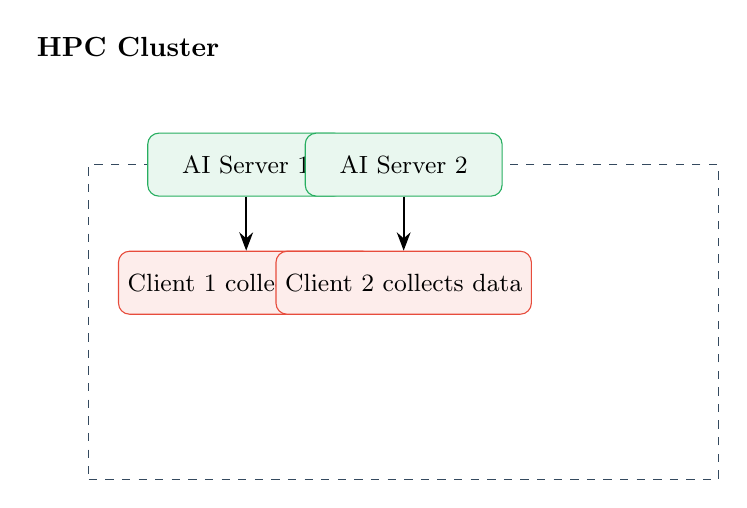
\begin{tikzpicture}[node distance=1.2cm]
    % HPC Cluster
    \node[container, minimum width=8cm, minimum height=4cm] (hpc) at (0, 0) {};
    \node at (-3.5, 3.5) {\textbf{HPC Cluster}};
    
    % Server nodes
    \node[server] (srv1) at (-2, 2) {AI Server 1};
    \node[server] (srv2) at (0, 2) {AI Server 2};
    
    % Client nodes with executors
    \node[client] (cli1) at (-2, 0.5) {Client 1 collects data};
    \node[client] (cli2) at (0, 0.5) {Client 2 collects data};
    
    % Connections
    \draw[arrow] (srv1) -- (cli1);
    \draw[arrow] (srv2) -- (cli2);
\end{tikzpicture}
\end{figure}

On the HPC cluster, each client computer has a small Python program that:
\begin{enumerate}
    \item Measures system performance (CPU, GPU, memory) every 1 second
    \item Stores these measurements in memory
    \item Provides them through a web endpoint on port 6000
\end{enumerate}

\subsection{Data Viewing on Your Laptop}

\begin{figure}[H]
\centering
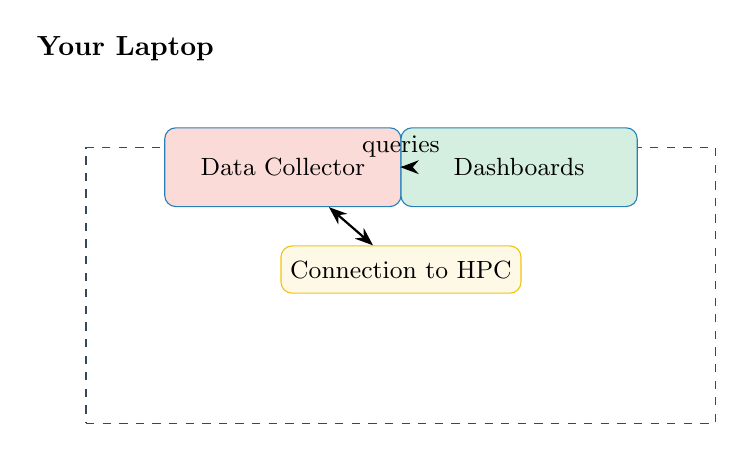
\begin{tikzpicture}[node distance=1.2cm]
    % Laptop
    \node[container, minimum width=8cm, minimum height=3.5cm] (laptop) at (0, 0) {};
    \node at (-3.5, 3) {\textbf{Your Laptop}};
    
    % Prometheus
    \node[component, fill=accent!20] (prom) at (-1.5, 1.5) {Data Collector};
    
    % Grafana
    \node[component, fill=success!20] (graf) at (1.5, 1.5) {Dashboards};
    
    % Tunnel
    \node[monitor, minimum height=0.6cm] (tunnel) at (0, 0.2) {Connection to HPC};
    
    % Connections
    \draw[biarrow] (prom) -- (tunnel);
    \draw[arrow] (prom) -- (graf) node[above, midway, font=\small] {queries};
\end{tikzpicture}
\end{figure}

On the laptop, there are two programs:

\begin{enumerate}
    \item \textbf{Prometheus} (on port 9092): A program that collects data from HPC every 15 seconds through the secure tunnel
    \item \textbf{Grafana} (on port 3001): A program that creates nice graphs from the collected data
\end{enumerate}

\subsection{Step-by-Step: From HPC to Your Dashboard}

\textbf{Step 1: HPC Client Collects Data}

On client computers on HPC, a Python monitor continuously runs:

\begin{lstlisting}[style=bash]
# Data is available here on HPC (inside the cluster)
http://client-node:6000/metrics/prometheus

# The data looks like:
ollama_throughput_rps 578           # 578 requests per second
ollama_workload_running 1           # 1 = workload is running
ollama_request_latency_seconds 0.015  # Each request takes 15ms
\end{lstlisting}

\textbf{Step 2: Create a Tunnel to HPC}

Since your laptop cannot directly see HPC, a secure tunnel is created:

\begin{lstlisting}[style=bash]
# Example: Create tunnel from your port 25000 to HPC client-node port 6000
ssh -N -L 25000:client-node:6000 meluxina &

# Now you can see HPC data from your laptop at:
http://localhost:25000/metrics/prometheus
\end{lstlisting}

\textbf{Step 3: Prometheus Reads the Data}

A program called Prometheus on your laptop reads from this tunnel:

\begin{lstlisting}[style=bash]
# Prometheus configuration file tells it where to look
# It checks every 15 seconds
scrape_configs:
  - job_name: 'ollama'
    static_configs:
      - targets: ['localhost:25000', 'localhost:25001']
\end{lstlisting}

\textbf{Step 4: Grafana Shows You the Graphs}

Grafana reads the stored data from Prometheus and shows nice graphs:

\begin{itemize}
    \item A number showing if the workload is running (0 means stopped, 1 means running)
    \item A line graph showing requests per second over time
    \item A line graph showing response time over time
    \item Counters showing total successes and failures
\end{itemize}

\subsection{What the Dashboards Show}

\textbf{Ollama Performance Dashboard}

This shows performance of the Ollama AI model:

\begin{itemize}
    \item \textbf{Is it Running?}: Shows 0 (stopped) or 1 (running)
    \item \textbf{Total Requests}: How many AI requests have been made (goes up over time)
    \item \textbf{Speed per Computer}: Shows requests/sec on each computer (line graph)
    \item \textbf{Total Speed}: Shows all requests/sec combined (big number)
    \item \textbf{Response Time}: How long each request takes (line graph in milliseconds)
    \item \textbf{Success vs Failure}: Comparison of successful vs failed requests (bar chart)
    \item \textbf{Error Percentage}: What percent of requests failed (line graph)
\end{itemize}

\textbf{vLLM Performance Dashboard}

Same metrics of the Ollama but for the vLLM AI model, with extra panels:

\begin{itemize}
    \item \textbf{Tokens per Request}: How many words the AI generates per request
    \item \textbf{Cache Usage}: How full the GPU cache is (as a percentage)
\end{itemize}

\subsection{SSH Tunneling for Metrics}
\begin{itemize}
    \item \textbf{Ollama Dashboard}: 13 panels monitoring Ollama workload metrics
    \begin{itemize}
        \item Workload Status (gauge: 0=idle, 1=running)
        \item Requests Total (counter)
        \item Throughput by Host (timeseries)
        \item Total Throughput (stat panel in RPS)
        \item Request Latency (timeseries in ms)
        \item Success vs Failed Requests (bar chart)
        \item Error Rate Over Time (percentage)
        \item Plus additional CPU/GPU/Memory panels
    \end{itemize}
    
    \item \textbf{vLLM Dashboard}: Same layout with vLLM-specific metrics
    \begin{itemize}
        \item vllm\_workload\_running
        \item vllm\_throughput\_rps
        \item vllm\_request\_latency\_seconds
        \item vllm\_tokens\_per\_request
        \item vllm\_cache\_usage
    \end{itemize}
\end{itemize}

\textbf{Example Grafana Queries:}
\begin{lstlisting}[style=bash]
# Current workload status
ollama_workload_running

# Throughput aggregated across hosts
sum(ollama_throughput_rps)

# Latency p95
histogram_quantile(0.95, ollama_request_latency_seconds)

# Error rate
100 * (sum(rate(ollama_errors_total[5m])) / sum(rate(ollama_requests_total[5m])))
\end{lstlisting}

\subsection{SSH Tunneling for Metrics Access}

\begin{enumerate}
    \item \textbf{Find client nodes from job output}:
    \begin{lstlisting}[style=bash]
ssh meluxina "scontrol show job JOBID | grep StdOut"
ssh meluxina "cat /path/to/logs/*.out" | grep "Client nodes"
    \end{lstlisting}
    
    \item \textbf{Open SSH tunnels}:
    \begin{lstlisting}[style=bash]
# Ollama clients
ssh -N -L 25000:mel2120:6000 meluxina &
ssh -N -L 25001:mel2148:6000 meluxina &

# vLLM clients
ssh -N -L 25002:mel2142:6000 meluxina &
ssh -N -L 25003:mel2185:6000 meluxina &
    \end{lstlisting}
    
    \item \textbf{Verify metrics endpoint}:
    \begin{lstlisting}[style=bash]
curl http://localhost:25000/metrics/prometheus | head -5
    \end{lstlisting}
    
    \item \textbf{Access Grafana}:
    \begin{lstlisting}[style=bash]
open http://localhost:3001  # admin / admin
    \end{lstlisting}
\end{enumerate}

% ============================================================================
\section{Benchmarking Implementation}
% ============================================================================

\begin{placeholder}{Laura's Section}
Please provide comprehensive documentation of the benchmarking system:

\subsection{Workload Executor Implementation}
\begin{itemize}
    \item Thread pool management
    \item Request generation
    \item Latency measurement
    \item Error handling
\end{itemize}

\subsection{Ollama Benchmarking}
\begin{itemize}
    \item HellaSwag dataset integration
    \item Request format
    \item Response parsing
    \item Metrics collection
\end{itemize}

\subsection{vLLM Benchmarking}
\begin{itemize}
    \item OpenAI-compatible API usage
    \item Streaming vs non-streaming
    \item Token counting
    \item Throughput calculation
\end{itemize}

\subsection{Metrics Collection}
\begin{itemize}
    \item Latency percentiles (p50/p90/p99)
    \item Throughput (requests/second, tokens/second)
    \item Error rates
    \item Resource utilization
\end{itemize}

\subsection{Load Patterns}
\begin{itemize}
    \item Constant load
    \item Poisson distribution
    \item Burst patterns
\end{itemize}

Please include:
\begin{itemize}
    \item Code snippets for key implementations
    \item Diagrams showing request flow
    \item Example metrics output
    \item Performance considerations
\end{itemize}
\end{placeholder}

% ============================================================================
\section{Logging System}
% ============================================================================

\begin{placeholder}{Giulia's Section}
Please provide comprehensive documentation of the logging system:

\subsection{Logging Architecture}
\begin{itemize}
    \item Overall logging design
    \item Log sources and destinations
    \item Aggregation strategy
\end{itemize}

\subsection{BaseLogCollector}
\begin{itemize}
    \item Abstract interface design
    \item LogSource dataclass
    \item Method specifications
\end{itemize}

\subsection{TailerLogCollector}
\begin{itemize}
    \item File tailing implementation
    \item Remote node log collection
    \item Log aggregation
\end{itemize}

\subsection{Log Categories}
\begin{itemize}
    \item Application logs
    \item System logs (Slurm)
    \item Benchmark logs
    \item Infrastructure logs
\end{itemize}

\subsection{Log Format and Storage}
\begin{itemize}
    \item Structured logging (JSON)
    \item Timestamps and correlation IDs
    \item Storage organization
    \item Retention policies
\end{itemize}

Please include:
\begin{itemize}
    \item TikZ diagrams for log flow
    \item Code snippets for key implementations
    \item Example log entries
    \item Integration with other components
\end{itemize}
\end{placeholder}

% ============================================================================
\section{CLI and User Interface}
% ============================================================================

\subsection{benchmark\_cli.py}

The main CLI provides three primary commands:

\begin{table}[H]
\centering
\begin{tabular}{@{}llp{8cm}@{}}
\toprule
\textbf{Command} & \textbf{Arguments} & \textbf{Description} \\
\midrule
\texttt{list} & -- & Display all available recipes with details \\
\texttt{create} & -- & Interactive wizard for recipe creation \\
\texttt{run} & \texttt{--recipe PATH} & Deploy and run a benchmark recipe \\
\bottomrule
\end{tabular}
\caption{CLI commands}
\end{table}

\subsection{Orchestrator Arguments}

\begin{lstlisting}[style=bash, caption={Orchestrator command-line arguments}]
python3 orchestrator.py \
  --server-nodes NODE [NODE ...]      # Required: Server hostnames
  --client-nodes NODE [NODE ...]      # Required: Client hostnames
  --workload-config-file PATH         # Required: Recipe file
  [--server-port PORT]                # Default: 11434/8000
  [--client-port PORT]                # Default: 5000
  [--timeout SECONDS]                 # Default: 600
  [--enable-monitoring]               # Enable metrics
  [--pushgateway-node NODE]           # For Prometheus
  [--monitor-interval SECONDS]        # Default: 5
  [--monitor-output PATH]             # Output file
\end{lstlisting}

\subsection{Interactive Recipe Creation}

The CLI guides users through recipe creation:

\begin{enumerate}
    \item Service selection (Ollama, vLLM, vLLM Distributed)
    \item Scenario configuration (name, partition, account)
    \item Node allocation (servers, clients, monitors)
    \item Resource requirements (GPUs, CPUs, memory)
    \item Workload parameters (model, duration, clients)
    \item Container paths and bind mounts
\end{enumerate}

% ============================================================================
\section{Slurm Integration}
% ============================================================================

\subsection{SBATCH Script Generation}

The toolkit generates Slurm batch scripts from recipes:

\begin{lstlisting}[style=bash, caption={Generated SBATCH script structure}]
#!/bin/bash
#SBATCH --job-name=ollama-benchmark
#SBATCH --partition=gpu
#SBATCH --account=p200981
#SBATCH --nodes=5
#SBATCH --time=02:00:00
#SBATCH --exclusive

# Load modules
module load Apptainer

# Get node list
NODES=($(scontrol show hostnames $SLURM_JOB_NODELIST))
SERVER_NODES="${NODES[0]} ${NODES[1]}"
CLIENT_NODES="${NODES[2]} ${NODES[3]}"
ORCHESTRATOR_NODE="${NODES[4]}"

# Start servers
for node in $SERVER_NODES; do
    srun --nodes=1 --nodelist=$node \
        apptainer run --nv ollama.sif &
done

# Wait for servers
sleep 30

# Start client executors
for node in $CLIENT_NODES; do
    srun --nodes=1 --nodelist=$node \
        apptainer exec python.sif \
        python3 executor.py --port 6000 &
done

# Run orchestrator
python3 orchestrator.py \
    --server-nodes $SERVER_NODES \
    --client-nodes $CLIENT_NODES \
    --workload-config-file recipe.yaml
\end{lstlisting}

\subsection{Resource Allocation}

\begin{figure}[H]
\centering
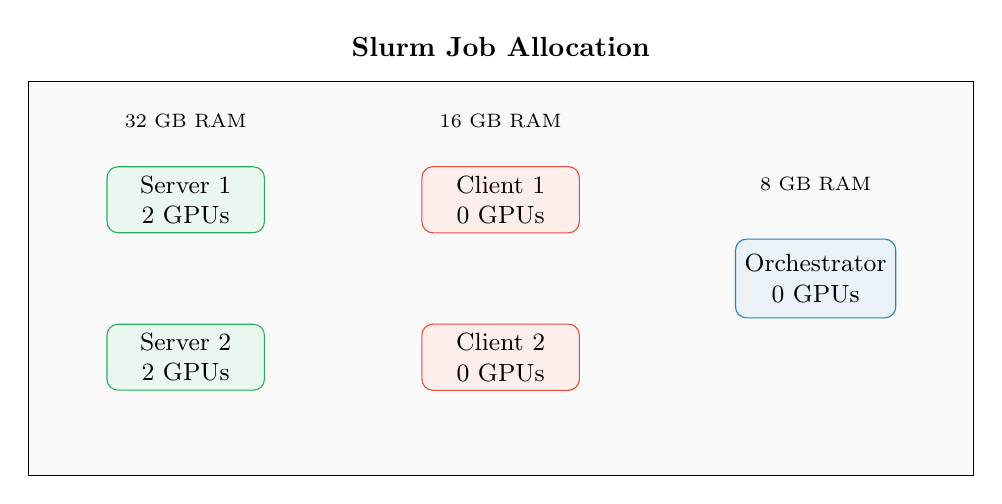
\begin{tikzpicture}[node distance=1cm]
    % Slurm allocation
    \node[draw, minimum width=12cm, minimum height=5cm, fill=gray!5] (slurm) at (0, 0) {};
    \node[above] at (0, 2.7) {\textbf{Slurm Job Allocation}};

    % Nodes
    \node[server, minimum width=2cm, align=center] (s1) at (-4, 1) {Server 1\\2 GPUs};
    \node[server, minimum width=2cm, align=center] (s2) at (-4, -1) {Server 2\\2 GPUs};
    \node[client, minimum width=2cm, align=center] (c1) at (0, 1) {Client 1\\0 GPUs};
    \node[client, minimum width=2cm, align=center] (c2) at (0, -1) {Client 2\\0 GPUs};
    \node[component, minimum width=2cm, align=center] (orch) at (4, 0) {Orchestrator\\0 GPUs};

    % Labels
    \node[font=\scriptsize] at (-4, 2) {32 GB RAM};
    \node[font=\scriptsize] at (0, 2) {16 GB RAM};
    \node[font=\scriptsize] at (4, 1.2) {8 GB RAM};
\end{tikzpicture}
\caption{Slurm resource allocation example}
\end{figure}

% ============================================================================
\section{Extensibility}
% ============================================================================

\subsection{Adding a New Service}

To add a new inference service, implement four components:

\begin{enumerate}
    \item \textbf{Server Manager}: Handle service lifecycle
    \item \textbf{Workload Controller}: Coordinate clients
    \item \textbf{Workload Executor}: Execute benchmarks
    \item \textbf{Service Registration}: Register with factory
\end{enumerate}

\begin{figure}[H]
\centering
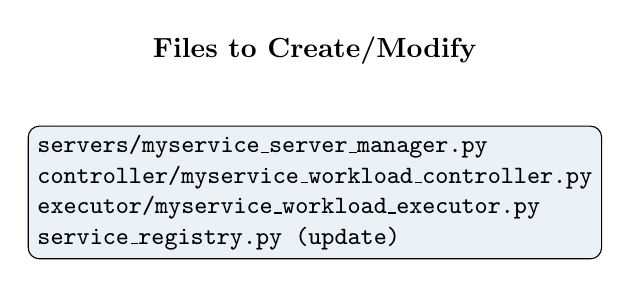
\begin{tikzpicture}[node distance=2cm]
    % Files to create
    \node[draw, rounded corners, fill=primary!10, minimum width=6cm, align=left, font=\small\ttfamily] (files) at (0, 0) {
        servers/myservice\_server\_manager.py \\
        controller/myservice\_workload\_controller.py \\
        executor/myservice\_workload\_executor.py \\
        service\_registry.py (update)
    };

    \node[above] at (0, 1.5) {\textbf{Files to Create/Modify}};
\end{tikzpicture}
\end{figure}

\subsection{Custom Metrics}

Extend the Monitor class for custom metrics:

\begin{lstlisting}[style=python, caption={Custom metrics extension}]
from prometheus_client import Gauge

class CustomMonitor(Monitor):
    def __init__(self, *args, **kwargs):
        super().__init__(*args, **kwargs)
        self.custom_metric = Gauge(
            'custom_metric',
            'Description of custom metric'
        )

    def collect_custom(self):
        value = self._get_custom_value()
        self.custom_metric.set(value)
\end{lstlisting}

% ============================================================================
\section{Deployment and Operations}
% ============================================================================

\subsection{Prerequisites}

\begin{table}[H]
\centering
\begin{tabular}{@{}lll@{}}
\toprule
\textbf{Component} & \textbf{Requirement} & \textbf{Version} \\
\midrule
Python & Runtime & 3.6+ \\
Slurm & Job scheduler & Any \\
Apptainer & Container runtime & 1.0+ \\
Docker & Local monitoring & 20.10+ \\
\bottomrule
\end{tabular}
\caption{System prerequisites}
\end{table}

\subsection{Python Dependencies}

\begin{lstlisting}[style=bash, caption={Required Python packages}]
pip install flask requests psutil prometheus_client pyyaml
\end{lstlisting}

\subsection{Container Setup}

\begin{lstlisting}[style=bash, caption={Building containers on MeluXina}]
module load Apptainer

# Pull Ollama container
apptainer pull docker://ollama/ollama:latest

# Pull vLLM container
apptainer pull docker://vllm/vllm-openai:latest

# Pull Python container for clients
apptainer pull docker://python:3.12.3-slim
\end{lstlisting}

% ============================================================================
\section{Performance Considerations}
% ============================================================================

\begin{placeholder}{Performance Analysis - Pending Laura's Benchmarking Results}
This section will be completed once Laura's benchmarking work is finalized. It will include:

\subsection{Bottleneck Analysis}
\begin{itemize}
    \item Latency breakdown for LLM inference
    \item GPU compute vs memory transfer analysis
    \item Network overhead measurements
    \item Tokenization performance impact
\end{itemize}

\subsection{Optimization Recommendations}
\begin{itemize}
    \item Warmup period requirements
    \item Batch size tuning guidelines
    \item Tensor parallelism configuration
    \item Memory utilization optimization
    \item Client concurrency tuning
\end{itemize}

\subsection{Scaling Analysis}
\begin{itemize}
    \item Single-node vs multi-node performance
    \item Strong scaling efficiency
    \item Weak scaling characteristics
    \item Resource utilization patterns
\end{itemize}

Please provide:
\begin{itemize}
    \item Benchmark results from Ollama and vLLM tests
    \item Performance charts and graphs
    \item Latency distributions (p50/p90/p99)
    \item Throughput measurements
    \item Resource utilization data
    \item Optimization recommendations based on findings
\end{itemize}
\end{placeholder}

% ============================================================================
\section{Troubleshooting Guide}
% ============================================================================

\subsection{Common Issues}

\begin{table}[H]
\centering
\begin{tabular}{@{}p{4cm}p{4cm}p{6cm}@{}}
\toprule
\textbf{Issue} & \textbf{Symptom} & \textbf{Solution} \\
\midrule
Server health check fails & Timeout during startup & Verify port accessibility, check container logs \\
Client cannot connect & Connection refused & Check executor is running, verify port \\
No metrics in Grafana & Empty dashboard & Verify SSH tunnel, check Prometheus targets \\
Ray cluster fails & Workers not connecting & Check network ports, verify head IP \\
\bottomrule
\end{tabular}
\caption{Common issues and solutions}
\end{table}

\subsection{Debugging Commands}

\begin{lstlisting}[style=bash, caption={Useful debugging commands}]
# Check server health
curl http://server-node:11434/api/tags

# Verify executor
curl http://client-node:6000/health

# Check Prometheus targets
curl http://localhost:9092/api/v1/targets

# View Ray cluster status
ssh head-node "ray status"
\end{lstlisting}

% ============================================================================
\section{Project Structure}
% ============================================================================

\begin{lstlisting}[style=bash, caption={Complete project structure}]
hpc-benchmark-toolkit/
+-- src/
|   +-- benchmark/
|   |   +-- orchestrator.py
|   |   +-- service_factory.py
|   |   +-- service_registry.py
|   |   +-- servers/
|   |   |   +-- base_server_manager.py
|   |   |   +-- ollama_server_manager.py
|   |   |   +-- vllm_server_manager.py
|   |   |   +-- ray_cluster_manager.py
|   |   +-- workload/
|   |   |   +-- controller/
|   |   |   +-- executor/
|   |   +-- logging/
|   +-- benchmark_cli.py
|   +-- monitor/
|       +-- monitor.py
+-- monitoring/
|   +-- docker-compose.yml
|   +-- prometheus.yml
|   +-- grafana/
+-- schemas/
|   +-- recipe-format.yaml
+-- docs/
+-- diagrams/
\end{lstlisting}

% ============================================================================
\section{Division of Work}
% ============================================================================

This section documents the contributions of each team member to the project.

\subsection{Alberto Finardi}

\textbf{Role}: System Architect and Service Implementation\\
\textbf{Contributions}:
\begin{itemize}
    \item \textbf{Core Architecture Design}
    \begin{itemize}
        \item Designed the overall system architecture
        \item Implemented the Service Factory pattern
        \item Created the modular component structure
    \end{itemize}

    \item \textbf{Server Management}
    \begin{itemize}
        \item Implemented \texttt{BaseServerManager} abstract class
        \item Developed \texttt{OllamaServerManager} with health checks and model pulling
        \item Developed \texttt{VllmServerManager} with distributed support
        \item Created \texttt{RayClusterManager} for distributed vLLM
    \end{itemize}

    \item \textbf{Workload Control}
    \begin{itemize}
        \item Designed \texttt{BaseWorkloadController} interface
        \item Implemented service-specific controllers
        \item Developed HTTP-based client coordination
    \end{itemize}

    \item \textbf{Workload Execution}
    \begin{itemize}
        \item Created \texttt{BaseWorkloadExecutor} Flask server
        \item Implemented REST API endpoints
        \item Developed thread pool management
    \end{itemize}

    \item \textbf{CLI Development}
    \begin{itemize}
        \item Developed \texttt{benchmark\_cli.py}
        \item Implemented interactive recipe creation wizard
        \item Created deployment and job submission logic
    \end{itemize}

    \item \textbf{Orchestration}
    \begin{itemize}
        \item Implemented main orchestrator logic
        \item Developed seven-phase execution model
        \item Created Slurm sbatch script generation
    \end{itemize}

    \item \textbf{Documentation}
    \begin{itemize}
        \item Wrote comprehensive README.md
        \item Created API Reference documentation
        \item Developed Developer Guide
        \item Authored this technical report
    \end{itemize}

    \item \textbf{Integration}
    \begin{itemize}
        \item Integrated all components
        \item Implemented service registry
        \item Coordinated team contributions
    \end{itemize}
\end{itemize}

\subsection{Giovanni}

\textbf{Role}: Monitoring

\begin{placeholder}{Giovanni's Contributions}
\begin{itemize}
    \item \textbf{Monitor Tool} (\texttt{src/monitor/monitor.py})
    \begin{itemize}
        \item Built a tool that measures CPU, GPU, and memory usage
        \item Runs in the background and checks every 1 second
        \item Saves all measurements to a CSV file for later analysis
        \item Works with Prometheus (data collection system) to send data to your laptop
        \item Supports computers with multiple GPUs
    \end{itemize}

    \item \textbf{Prometheus Setup}
    \begin{itemize}
        \item Set up Prometheus Pushgateway (a storage box for metric data)
        \item Made data format that Prometheus understands
        \item Made it so data is sent every 15 seconds to storage
        \item Created the configuration file (\texttt{monitoring/prometheus.yml})
        \item Made metrics available on port 6000 on each client computer
    \end{itemize}

    \item \textbf{Grafana Dashboards}
    \begin{itemize}
        \item Docker setup for Grafana (dashboard program)
        \item Designed and built two dashboards (one for Ollama, one for vLLM)
        \item Each dashboard has 13 different graphs and numbers
        \item Graphs show: requests per second, response time, success vs failure, errors
        \item Made it so you can see data from each computer separately or all together
        \item Made dashboards refresh automatically to show live data
    \end{itemize}

    \item \textbf{Docker Monitoring Stack}
    \begin{itemize}
        \item Set up Docker containers for Prometheus, Grafana, and storage
        \item Made sure data is saved even if you restart
        \item Made Grafana automatically load the dashboards
        \item Created a simple script (\texttt{monitoring/start.sh}) to start everything with one command
    \end{itemize}

    \item \textbf{SSH Tunnels for Secure Connection}
    \begin{itemize}
        \item Wrote guides explaining how to create secure connections from your laptop to HPC
        \item Set up port numbers (25000-25001 for Ollama, 25002-25003 for vLLM)
        \item Made it easy to find which computers to connect to from the job logs
        \item Wrote solutions for common connection problems
    \end{itemize}

    \item \textbf{Documentation}
    \begin{itemize}
        \item Created \texttt{monitoring/QUICKSTART.md} with step-by-step setup guide
        \item Wrote Phase 3 (Monitoring Setup) execution flow description
        \item Provided comprehensive Prometheus query examples and dashboard configuration details
    \end{itemize}
\end{itemize}
\end{placeholder}

\subsection{Laura}

\textbf{Role}: Validation \& Benchmarking

\begin{placeholder}{Laura's Contributions}
Please list your specific contributions:
\begin{itemize}
    \item \textbf{Recipe Validation}
    \begin{itemize}
        \item JSON Schema design (recipe-format.yaml)
        \item Validation logic implementation
        \item Custom validators
        \item Error message formatting
    \end{itemize}

    \item \textbf{Benchmarking Logic}
    \begin{itemize}
        \item Workload executor implementations
        \item Request generation logic
        \item Latency measurement
        \item Metrics aggregation
    \end{itemize}

    \item \textbf{Load Patterns}
    \begin{itemize}
        \item Constant load implementation
        \item Poisson distribution
        \item Burst patterns
    \end{itemize}

    \item \textbf{Documentation}
    \begin{itemize}
        \item Recipe guide contributions
        \item Benchmarking section of this report
    \end{itemize}
\end{itemize}
\end{placeholder}

\subsection{Giulia}

\textbf{Role}: Logging

\begin{placeholder}{Giulia's Contributions}
Please list your specific contributions:
\begin{itemize}
    \item \textbf{Logging Architecture}
    \begin{itemize}
        \item Log collector design
        \item Aggregation strategy
    \end{itemize}

    \item \textbf{BaseLogCollector}
    \begin{itemize}
        \item Abstract interface implementation
        \item LogSource dataclass design
    \end{itemize}

    \item \textbf{TailerLogCollector}
    \begin{itemize}
        \item File tailing implementation
        \item Remote log collection
    \end{itemize}

    \item \textbf{Log Management}
    \begin{itemize}
        \item Structured logging format
        \item Storage organization
        \item Correlation ID implementation
    \end{itemize}

    \item \textbf{Documentation}
    \begin{itemize}
        \item Logging section of this report
    \end{itemize}
\end{itemize}
\end{placeholder}

\subsection{Contribution Summary}

\begin{table}[H]
\centering
\begin{tabular}{@{}llp{6cm}@{}}
\toprule
\textbf{Team Member} & \textbf{Primary Area} & \textbf{Key Deliverables} \\
\midrule
Alberto Finardi & Architecture \& Core & Orchestrator, Server Managers, Controllers, Executors, CLI, Documentation \\
Giovanni & Monitoring & Monitor module, Prometheus/Grafana, Dashboards \\
Laura & Validation \& Benchmarking & Recipe validation, Workload execution, Metrics \\
Giulia & Logging & Log collectors, Aggregation, Storage \\
\bottomrule
\end{tabular}
\caption{Team contribution summary}
\end{table}

% ============================================================================
\section{Conclusion}
% ============================================================================

The HPC Benchmark Toolkit provides a comprehensive solution for benchmarking LLM inference services on HPC clusters. Key achievements include:

\begin{itemize}
    \item \textbf{Modular Architecture}: Clean separation of concerns with factory pattern
    \item \textbf{Multi-Service Support}: Ollama, vLLM (single and distributed)
    \item \textbf{Real-Time Monitoring}: Full Prometheus/Grafana integration
    \item \textbf{Reproducibility}: YAML-based recipe system
    \item \textbf{Extensibility}: Easy addition of new services
    \item \textbf{HPC Integration}: Native Slurm and Apptainer support
\end{itemize}

\subsection{Future Work}

Potential enhancements include:
\begin{itemize}
    \item Support for additional inference services (TensorRT, Triton)
    \item Kubernetes orchestration mode
    \item Automated performance regression testing
    \item Interactive web dashboard
    \item Multi-cluster support
\end{itemize}

% ============================================================================
% Appendices
% ============================================================================

\appendix

\section{Port Reference}

\begin{table}[H]
\centering
\begin{tabular}{@{}lll@{}}
\toprule
\textbf{Port} & \textbf{Service} & \textbf{Description} \\
\midrule
11434 & Ollama & Default Ollama API \\
8000 & vLLM & Default vLLM API \\
5000/6000 & Executor & Workload executor Flask \\
9091 & Pushgateway & Prometheus Pushgateway \\
9092 & Prometheus & Prometheus server \\
3001 & Grafana & Grafana dashboard \\
6379 & Ray & Ray cluster communication \\
8265 & Ray Dashboard & Ray monitoring \\
8076 & Ray Object Manager & Ray object store \\
8077 & Ray Node Manager & Ray node management \\
\bottomrule
\end{tabular}
\caption{Complete port reference}
\end{table}

\section{Environment Variables}

\begin{table}[H]
\centering
\begin{tabular}{@{}lll@{}}
\toprule
\textbf{Variable} & \textbf{Description} & \textbf{Default} \\
\midrule
PYTHONPATH & Python module path & -- \\
MLUX\_USER & MeluXina username & -- \\
MLUX\_ACCOUNT & MeluXina project account & -- \\
MLUX\_KEY & Path to SSH key & \textasciitilde/.ssh/id\_ed25519\_mlux \\
\bottomrule
\end{tabular}
\caption{Environment variables}
\end{table}

\end{document}
